\clearpage
%%=========================================
\section{Surface Analysis of As-Received Substrate C}\label{sec:subCa}
% Substrate C

Bright and dark field images of the as-received (211)B-oriented substrate C show that there are some large particles of size \SI{\sim 300}{\micro\metre} distributed sparsely over the substrate surface and that there are some smaller particles of size \SIrange{1}{15}{\micro\metre} with a somewhat larger density. Fig.~\ref{fig:subCa_om_bf} and Fig.~\ref{fig:subCa_om_df} displays the same location on the sample in bright field and dark field microscopy respectively. It is easier to see the particles in the dark field image, but they appear larger than they do in the bright field image.

\begin{figure}[htbp]
    \centering
    \mySubfigure{0.49\linewidth}{om_bf_subC_09_5x.jpg}[fig:subCa_om_bf]
    \hfill
    \mySubfigure{0.49\linewidth}{om_df_subC_07_5x.jpg}[fig:subCa_om_df]
    \caption[Bright and dark field optical microscopy images of as-received substrate C.]{Optical microscopy images of as-received substrate C taken at the same location on the substrate surface at a magnification of $5\times$: \subref{fig:subCa_om_bf} Bright field; and \subref{fig:subCa_om_df} dark field. The same particle configuration can be observed in both images.}
    \label{fig:subCa_om}
\end{figure}


\Ac{sem} images reveal that there are even smaller particles with lengths of \SIrange{30}{100}{\nano\metre} on the substrate surface. The small particles are distributed evenly over the surface. A typical area in the centre of substrate C can be seen in Fig.~\ref{fig:subCa_sem_area}. The particle density was found to be between \SI{2e+06}{\particle\centi\metre^{-2}} and \SI{1e+08}{\particle\centi\metre^{-2}}. The mean particle density was \SI{4e+07}{\particle\centi\metre^{-2}} with a standard deviation of \SI{2e+07}{\particle\centi\metre^{-2}}. A graphical representation of the particle density at different locations on substrate C can be seen in Fig.~\ref{fig:subCa_densityData}.

\begin{figure}[htbp]
    \centering
    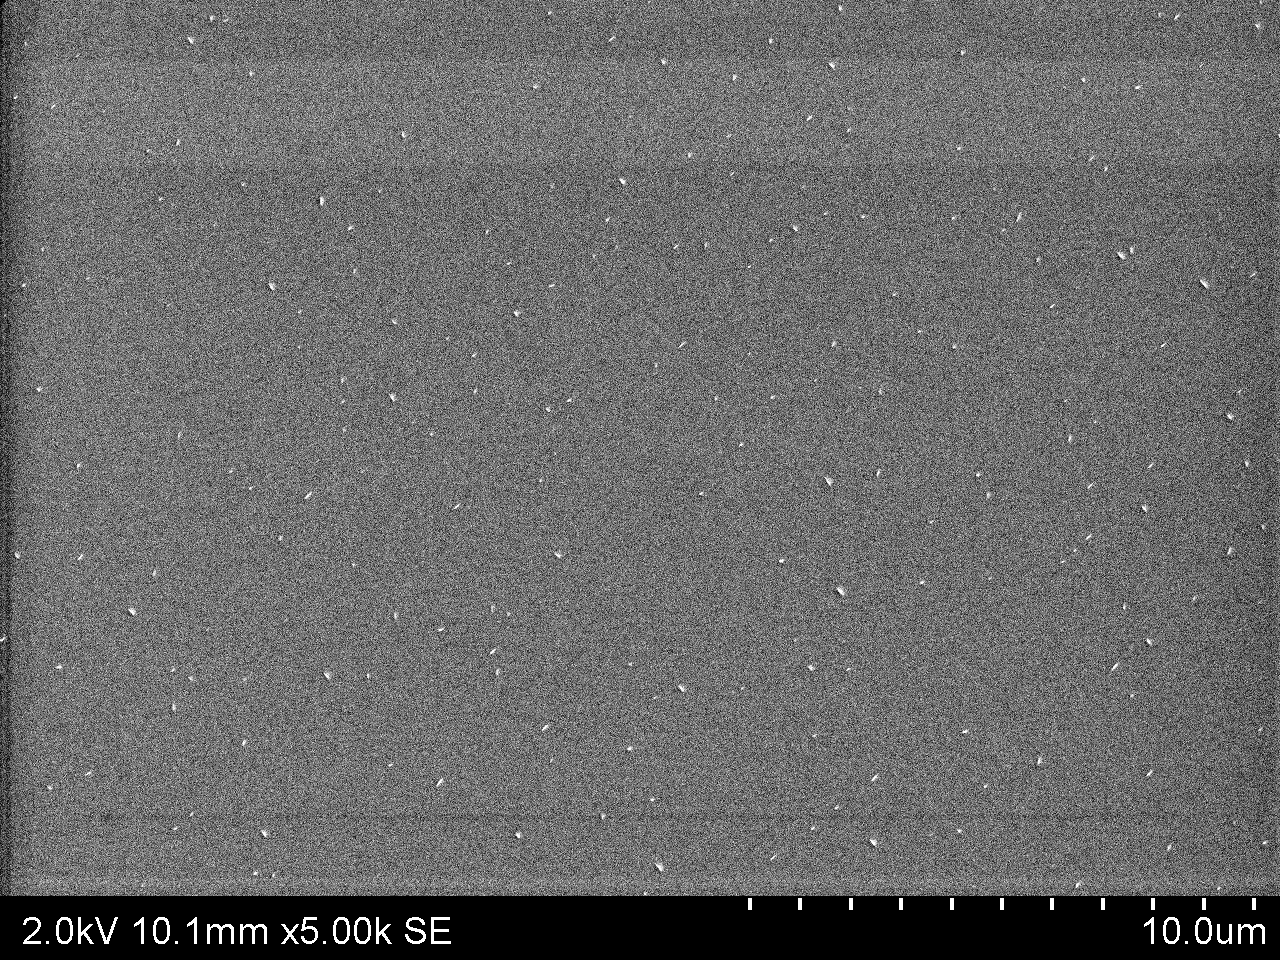
\includegraphics[width=1.0\linewidth]{sem_subCa_03_m005.png}
    \caption[\Ac{sem} image taken near the centre of the as-received substrate C.]{\Acf{sem} image taken near the centre of the as-received substrate C at a  magnification of $5000\times$.}
    \label{fig:subCa_sem_area}
\end{figure}

\begin{figure}[htbp]
    \centering
    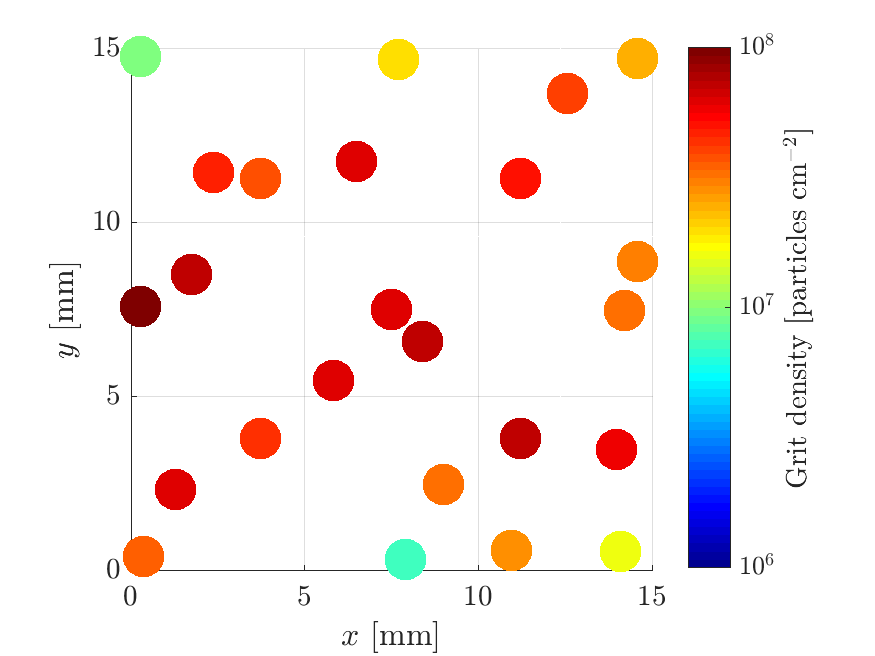
\includegraphics[width=0.7\linewidth]{subCa_densityData.png}
    \caption[Map of the polishing grit density on the as-received substrate C.]{A map of the polishing grit density at 24 different locations on the as-received $\SI{15}{\milli\metre}\times\SI{15}{\milli\metre}$ substrate C. The polishing grit density was observed to vary between \SI{2e+06}{\particle\centi\metre^{-2}} and \SI{1e+08}{\particle\centi\metre^{-2}}.}
    \label{fig:subCa_densityData}
\end{figure}

An \ac{eds} spectrum of one of the particles reveals that the piece is composed of silica oxide, \ce{SiO2}, also known as silica, see Fig.~\ref{fig:subCa_polishing-grit}. The \ac{sem} image displays an agglomeration of particles with a diameter of \SI{50}{\nano\metre}. The presence of silica can be explained by the frequent use of silica as an abrasive in polishing slurries for semiconducting material. The corresponding \ac{sem} image of residual polishing grit is shown next to the spectrum. The \ce{Al} contamination that can be seen in the \ac{eds} spectrum obtained from a large area of the substrate can come from residual \ce{Al2O3} polishing grit, also known as alumina. Due to the small extent of the individual residual particles, it was not possible to get \ac{eds} spectra from them unless multiple particles formed a larger pile, which was rarely observed.

\begin{figure}
    \centering
    \begin{subfigure}[t]{\textwidth}
          \begin{minipage}[t]{0.4\linewidth}
            \centering
            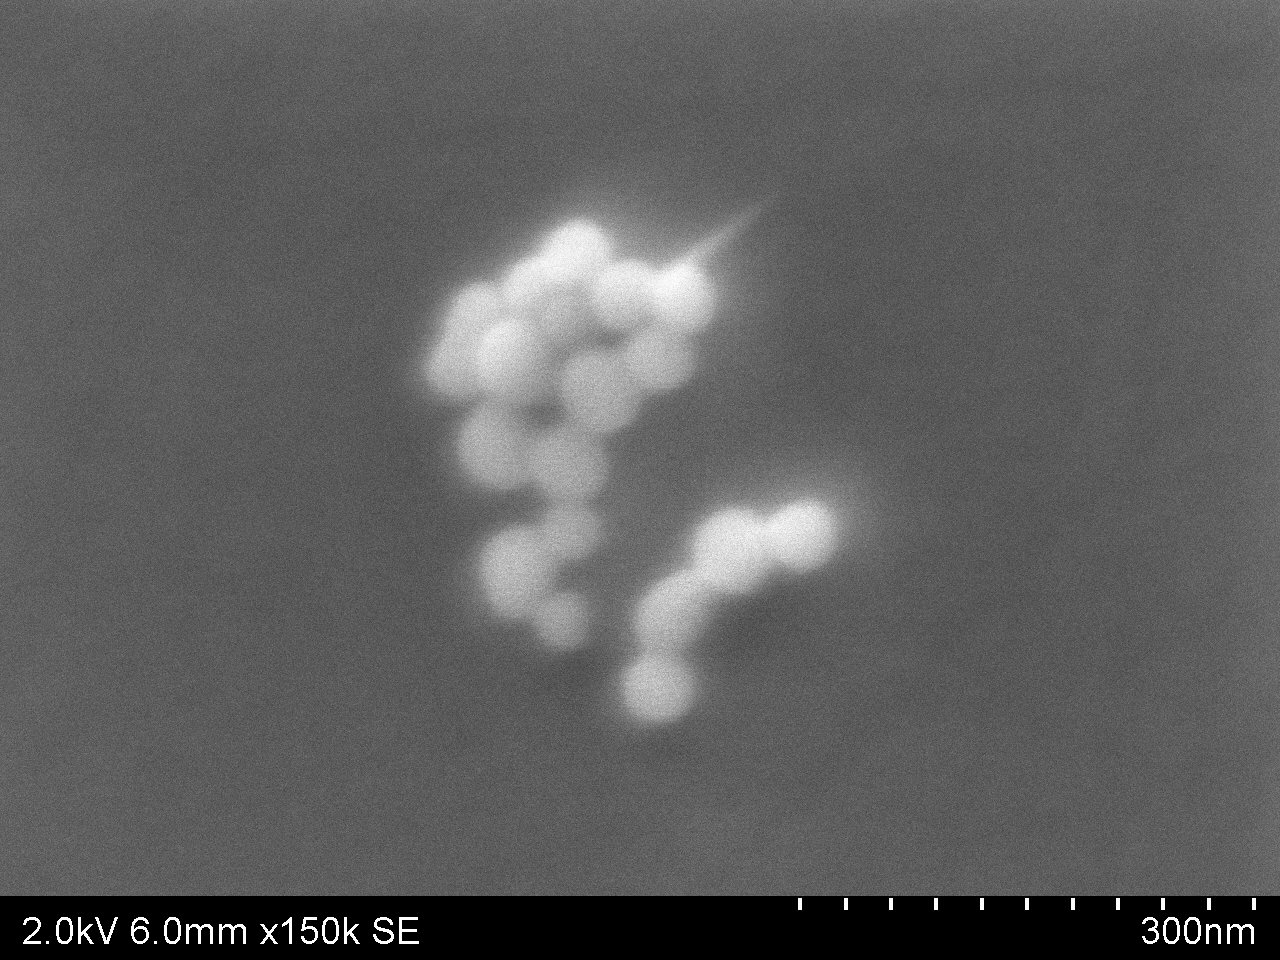
\includegraphics[width=\linewidth]{subCa_sem_09_m010.jpg}
          \end{minipage}
          \hfill
          \begin{minipage}[t]{0.56\linewidth}
            \centering
            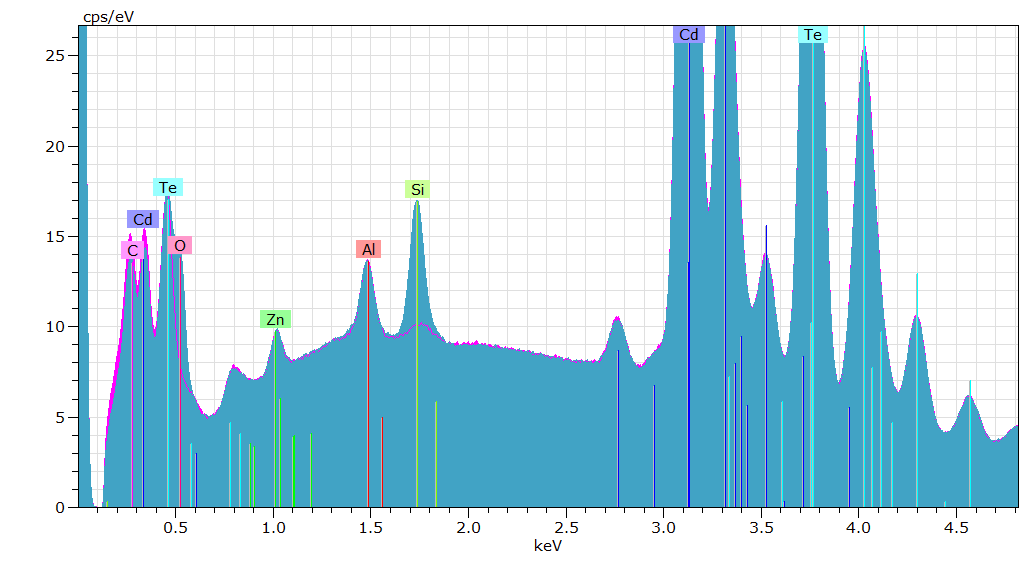
\includegraphics[width=\linewidth]{subCa_eds_s.png}
          \end{minipage}
        \caption{}\label{fig:subCa_polishing-grit}
    \end{subfigure}%
    \caption[\Ac{sem} images and \ac{eds} spectra of particles found on as-received substrate C.]{High resolution \acf{sem} images of particles found on the as-received substrate C and the corresponding \acf{eds} spectra of the particles: \subref{fig:subCa_polishing-grit} silica (\ce{SiO2}), the blue spectrum represents the measurements from the particles, while the pink spectrum represents the substrate surface next to the particles.}\label{fig:subCa_sem_w_eds}
\end{figure}

The large particles observed in the dark field images \todo{sett inn sem-bilde og eds-spektrum.}

%%=========================================
%\section{AFM Study of As-Received Substrate C}
\subsection{Surface Roughness}
The as-received substrate C was characterised for surface topography by \ac{afm}. \Ac{afm} images of the substrate surface are shown in Fig.~\ref{fig:subCa_afm}. Polishing grit particles can be observed all over the surface of the substrate. The typical polishing grit density on the (211)B-oriented substrate is \SI{\sim 6e7 }{\particle\centi\metre^{-2}}. The typical polishing grit length is \SIrange{50}{200}{\nano\metre} and the typical height was measured to be \SI{\sim 10}{\nano\metre} above the (211)B surface. The small height above the surface in comparison with the diameter of the particles indicates that the polishing grit particles have penetrated the surface and are partly included in the surface.

Fig.~\ref{fig:sem-afm-comparison} show a comparison of an \ac{afm} image with a \ac{sem} image taken at the same location on the as-received substrate C. The same particle configuration can be seen in both images, but the shape and size of the polishing grit particles observed in \ac{afm} are different to what were observed in the \ac{sem} images. This image artifact in the \ac{afm} image can be explained by the convolution effect between the tip and the polishing grit particles, as described in Section~\ref{sec:afm}. In other words, due to a too-course tip, an image artifact occur in the \ac{afm} image that makes the particles look wider and longer than they are. 

\begin{figure}[htbp]
    \centering
    \begin{subfigure}[t]{0.3\linewidth}
    \centering
        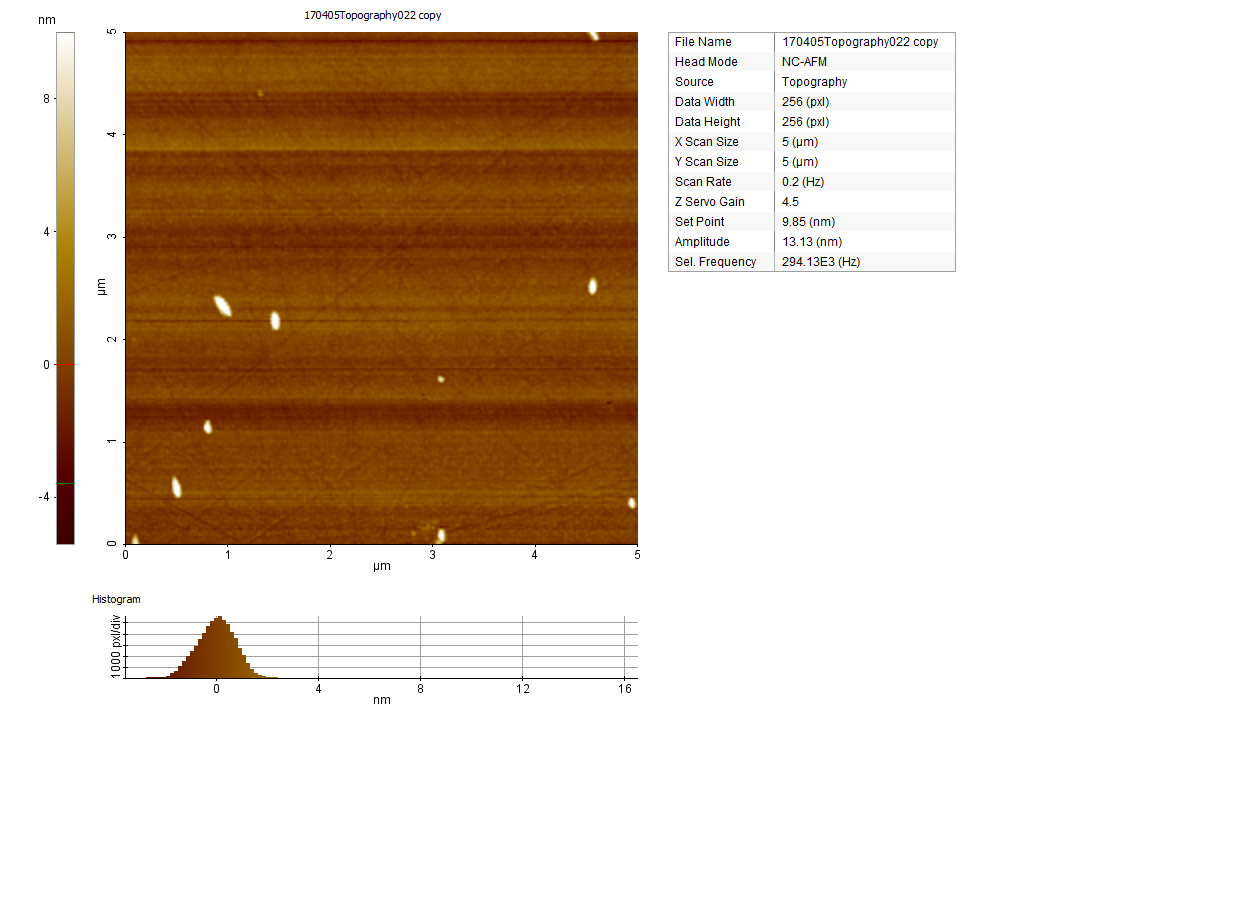
\includegraphics[width=\linewidth,trim={0cm 12cm 21cm 0cm},clip]{170405Topography022.png}
        \caption{}%0,33\SI{0,28}{\nano\metre}
        \label{fig:subCa_afm_centre}
    \end{subfigure}
    \hfill
    \begin{subfigure}[t]{0.3\linewidth}
    \centering
        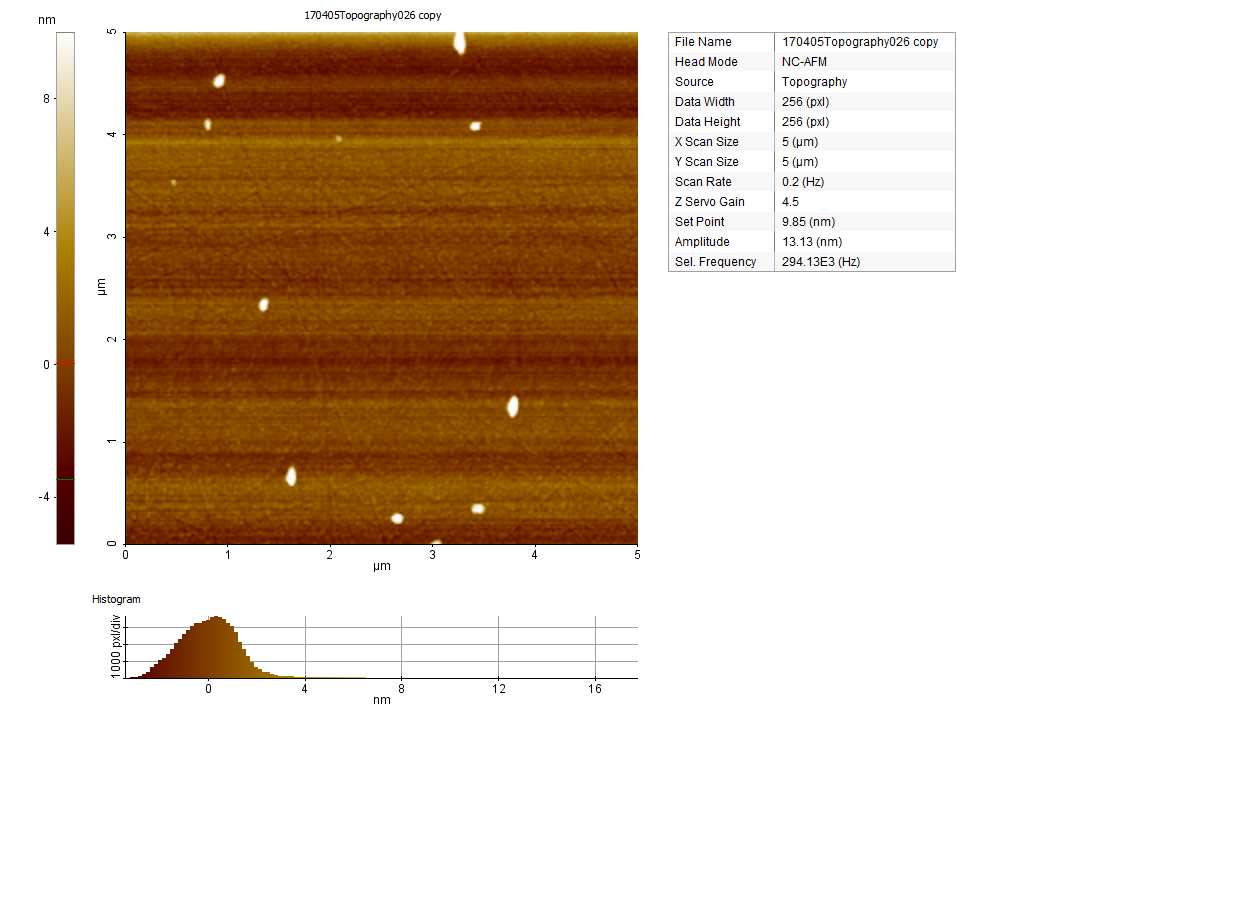
\includegraphics[width=\linewidth,trim={0cm 12cm 21cm 0cm},clip]{170405Topography026.png}
        \caption{}%0,46 \SI{0,36}{\nano\metre}
        \label{fig:subCa_afm_edge}
    \end{subfigure}
    \hfill
    \begin{subfigure}[t]{0.3\linewidth}
    \centering
        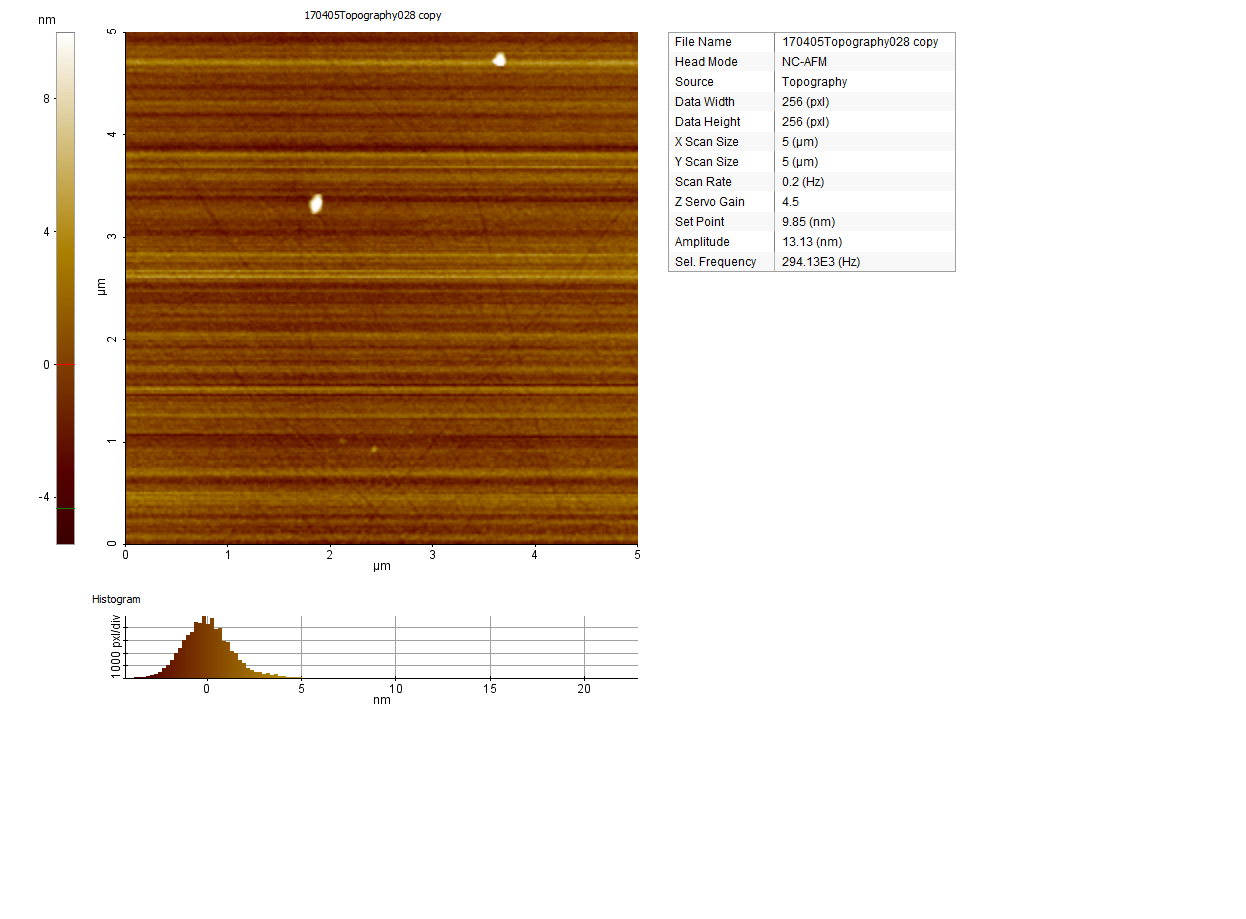
\includegraphics[width=\linewidth,trim={0cm 12cm 21cm 0cm},clip]{170405Topography028.png}
        \caption{}% 0.54\SI{0,40}{\nano\metre}
        \label{fig:subCa_afm_corner}
    \end{subfigure}
    \caption[\Ac{afm} of as-received substrate C.]{\Acf{afm} measurements of the as-received substrate C. Images of $\SI{5}{\micro\metre}\times\SI{5}{\micro\metre}$ areas are taken at three different locations on the substrate surface: \subref{fig:subCa_afm_centre} near the centre, \ac{rms} roughness \SI{0.95}{\nano\metre}; \subref{fig:subCa_afm_edge} near the left edge, \ac{rms} roughness \SI{1.4}{\nano\metre}; and \subref{fig:subCa_afm_corner} near the upper left corner, \ac{rms} roughness \SI{1.4}{\nano\metre}.}
    \label{fig:subCa_afm}
\end{figure} % AFM, substrate C, as-received.

%\todo{rar forklaring?}
To obtain a more accurate comparison of \ac{rms} roughness that is independent of polishing grit density, the measurements were performed on areas where there was no polishing grit. The averages of several such measurements made within the same image resulted in \iac{rms} roughness of \SI{\sim 0,3}{\nano\metre} at the centre and \SI{\sim 0.5}{\nano\metre} around the edges. \citet{benson2015as-received} determined a similar \ac{rms} roughness of \SI{\sim 0.4}{\nano\metre} on all the as-received (211)B-oriented \ac{czt} substrates they studied.\todo{Det er de som står prosenta ut i figuren over.}

The low \ac{rms} roughness indicates the absence of deep scratches. The deepest observed polishing scratches on substrate C are \SI{0,2}{\micro\metre} wide and only \SI{1}{\nano\metre} deep. 

\begin{figure}[htbp]
    \centering
    \begin{subfigure}[t]{0.45\linewidth}
        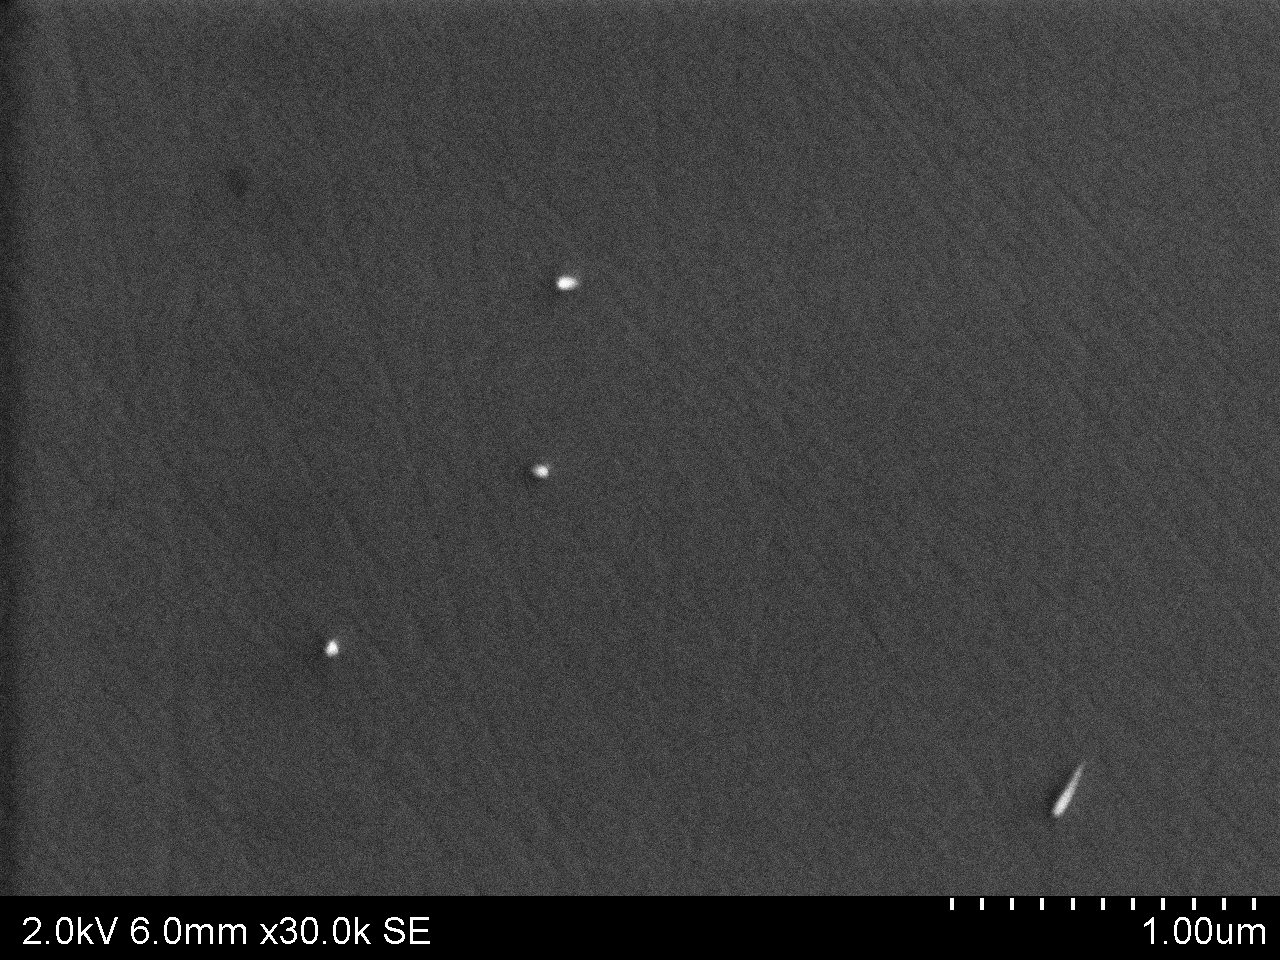
\includegraphics[width=\linewidth]{subCa_sem_afm_compare_m010.jpg}
        \caption{}\label{fig:sem-afm-comparison_sem}
    \end{subfigure}%
    \begin{subfigure}[t]{0.45\linewidth}
        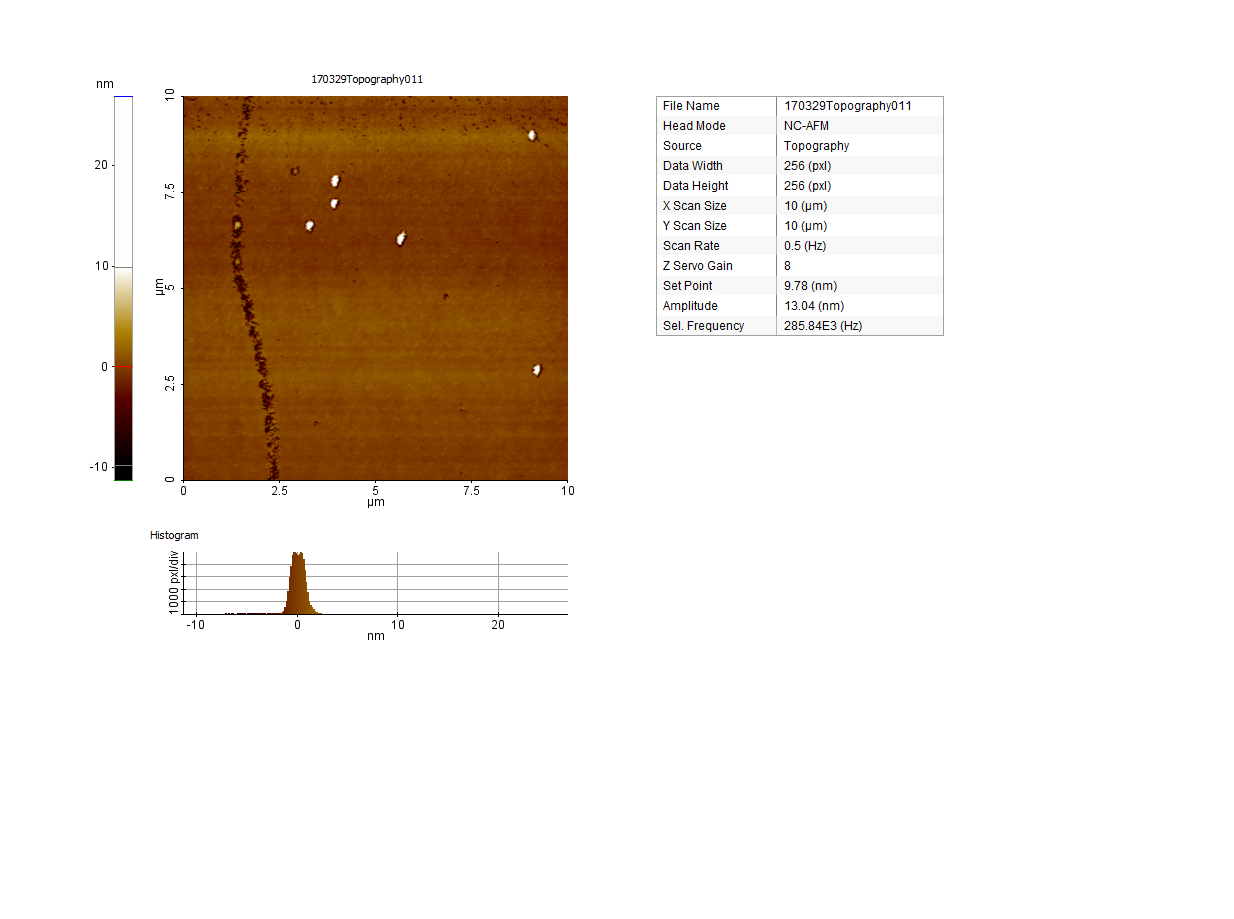
\includegraphics[width=\linewidth,trim={2.5cm 14.5cm 23cm 1.5cm},clip]{subCa_afm_lysmikrokopi05_afm02.png}
        \caption{}\label{fig:sem-afm-comparison_afm}
    \end{subfigure}%
    \caption[Comparison of an \ac{afm} image with a \ac{sem} image taken at the same location on substrate C.]{Comparison of \subref{fig:sem-afm-comparison_sem} a \ac{sem} image with \subref{fig:sem-afm-comparison_afm} an \ac{afm} image taken at the same location on the as-received substrate C. The height of the features in the \ac{afm} image is displayed as colour gradations. The same location with the same particles can be seen in both the \ac{afm} image and the \ac{sem} image, but due to a too-course tip, an image artifact occur in the \ac{afm} image that makes the particles look wider and longer than they are. The advantage of the \ac{afm} image is that it gives height information.}
    \label{fig:sem-afm-comparison}
\end{figure}

%\todo{Hvorfor er størrelsen og formen på partiklene sett med AFM helt ulik det sett i SEM? Er det to ulike typer partikler? Og i så fall, hvorfor ser jeg ikke poleringspartiklene i AFM? Og hvorfor ser jeg ikke hulrom med partikkel i midten i SEM? Er gropene for grunne (10 nm) til at de kan sees i SEM? Eller er det avbildingsfeil i AFM?}
%\begin{itemize}
%    \item \todo{Teori 1: To typer. AFM dytter vekk poleringspartiklene, SEM kan ikke se så grunne hulrom.}
%    \item \todo{Teori 2: Én type. AFM dytter vekk poleringspartiklene, det vi ser er slik det ser ut under poleringspartiklene. Denne teorien støttes av at alle gropene peker i samme retning.}
%    \item \todo{Teori 3: Én type. Det er samme type partikler vi ser i både SEM og AFM, men pga. avbildningsfeil i AFM, oppfattes de annerledes.}
%\end{itemize}

%%=========================================
\subsection{Impurity Analysis}

\Ac{eds} impurity analysis was performed on the as-received substrate C. Three locations on the surface -- the centre, the edge, and the corner -- were analysed. The results of this analysis can be seen in Table~\ref{tab:subCa_eds_analysis}. The only elements found above the \ac{eds} detection limit, in addition to \ce{Cd}, \ce{Zn}, and \ce{Te}, were \ce{Al}, \ce{Si}, \ce{C}, and \ce{O}.

\begin{table}[htbp]
    \centering
    \caption[\Ac{eds} impurity analysis of the as-received substrate C.]{Results of the \acf{eds} impurity analysis at three different locations on the $15\times15$ \SI{}{\milli\metre^2} as-received (211)B \ac{czt} substrate C (atomic concentration \%). The X-ray signal is acquired from a $\SI{1270}{}\times\SI{890}{\micro\metre^2}$ area centred around the given $X$ and $Y$ values at a magnification of 100$\times$.}\label{tab:subCa_eds_analysis}
    \begin{tabu} to 1.0\textwidth { X[1,c] X[1,c] X[1.125,c] X[1.125,c] X[1.125,c] X[1.125,c] X[1.125,c] X[1.125,c] X[1.125,c] }
    \hline
        \textbf{$X$} (\SI{}{\milli\metre}) &  \textbf{$Y$} (\SI{}{\milli\metre}) & \textbf{\ce{Te}} (at.\%) & \textbf{\ce{Cd}} (at.\%) & \textbf{\ce{Zn}} (at.\%) & \textbf{\ce{Al}} (at.\%) & \textbf{\ce{Si}} (at.\%) & \textbf{\ce{C} } (at.\%) & \textbf{\ce{O}} (at.\%) \\
        \hline
         \SI{1.0}{} & \SI{14.0}{} & \SI{45.05}{}& \SI{45.09}{} & \SI{1.44}{} & \SI{2.00}{}& \SI{0.46}{} & \SI{4.83}{} & \SI{1.13}{} \\
         \SI{7.5}{} & \SI{14.0}{} & \SI{45.09}{}& \SI{45.09}{} & \SI{1.49}{} & \SI{1.70}{}& \SI{0.46}{} & \SI{4.93}{} & \SI{1.23}{}  \\
         \SI{7.5}{} & \SI{7.5}{}  & \SI{44.85}{}& \SI{44.90}{} & \SI{1.44}{} & \SI{1.98}{}& \SI{0.51}{} & \SI{4.93}{} & \SI{1.40}{}  \\
         \hline
    \end{tabu}
\end{table}

%%=========================================
%\section{Near-IR of As-Received Substrate C}

Near-\ac{ir} transmission microscopy images of as-received substrate C show a structure that has not appeared on either optical microscopy, \ac{sem}, or \ac{afm}. The structures are closed loops -- both circular loops and buckled loops with more curvature -- that appear brighter than the surrounding substrate, see Fig.~\ref{fig:subCa_irt}. The fact that the loops are brighter indicates that more of the photons are transmitted through.

\begin{figure}[htbp]
    \centering
    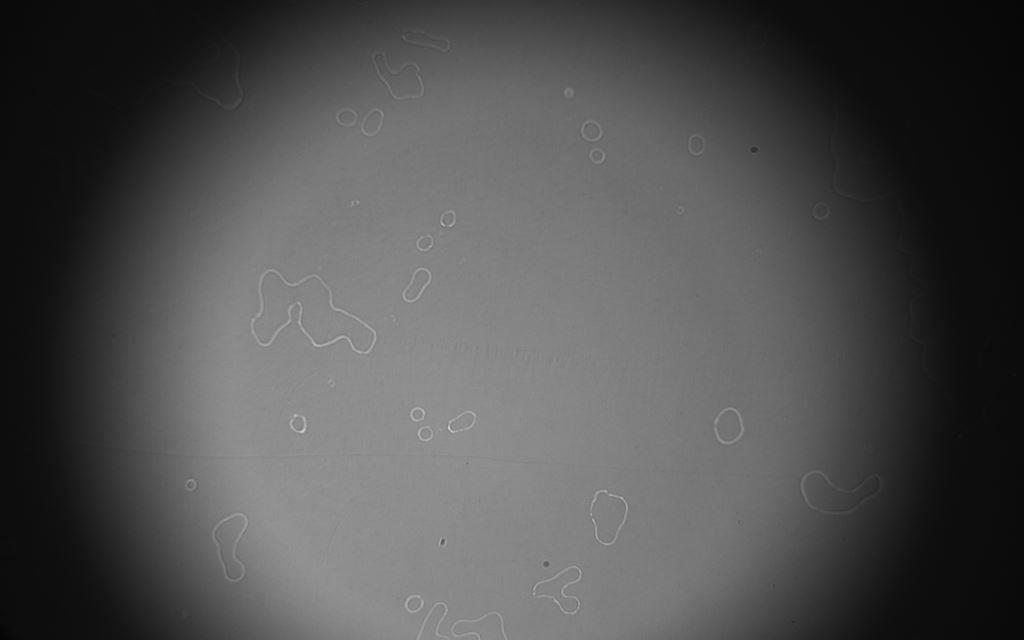
\includegraphics[width=1.0\linewidth]{ir_20170210_038.jpg}
    \caption[Near-\ac{ir} transmission microscopy of as-received substrate C.]{Near-\ac{ir} transmission microscopy images of as-received substrate C taken near the lower left corner.}
    \label{fig:subCa_irt}
\end{figure}

%%=========================================
% FTIR transmission spectra
\subsection{IR Characterisation}

\Ac{ftir} transmission spectra were recorded from a $5\times5$ grid on the as-received substrate C. The grid points were placed \SI{2.3}{\milli\metre} from the edge and had \SI{2.6}{\milli\metre} between nearest neighbours. All but five measurements had an \ac{ir} transmittance between \SI{62}{\percent} and \SI{67}{\percent} in the wavenumber range between \SI{500}{\centi\metre^{-1}} and \SI{5000}{\centi\metre^{-1}}, see Fig.~\ref{fig:subCa_ftir_spectra}. The indicator $T_{1000}/T_{5000}$ was a little bit less than one for these points. According to \citet{yujie2004infrared}, the \ac{czt} substrates with these characteristics are free of precipitates, have low free carrier concentration, and have resistivity that exceeds \SI{e6}{\ohm\centi\metre}. A map of the transmission at $k=\SI{500}{\centi\metre^{-1}}$ can be seen in Fig.~\ref{fig:subCa_ftir_map_500cm-1}.

\begin{figure}[htbp]
    \centering
    \begin{subfigure}[t]{0.60175438596\linewidth}
        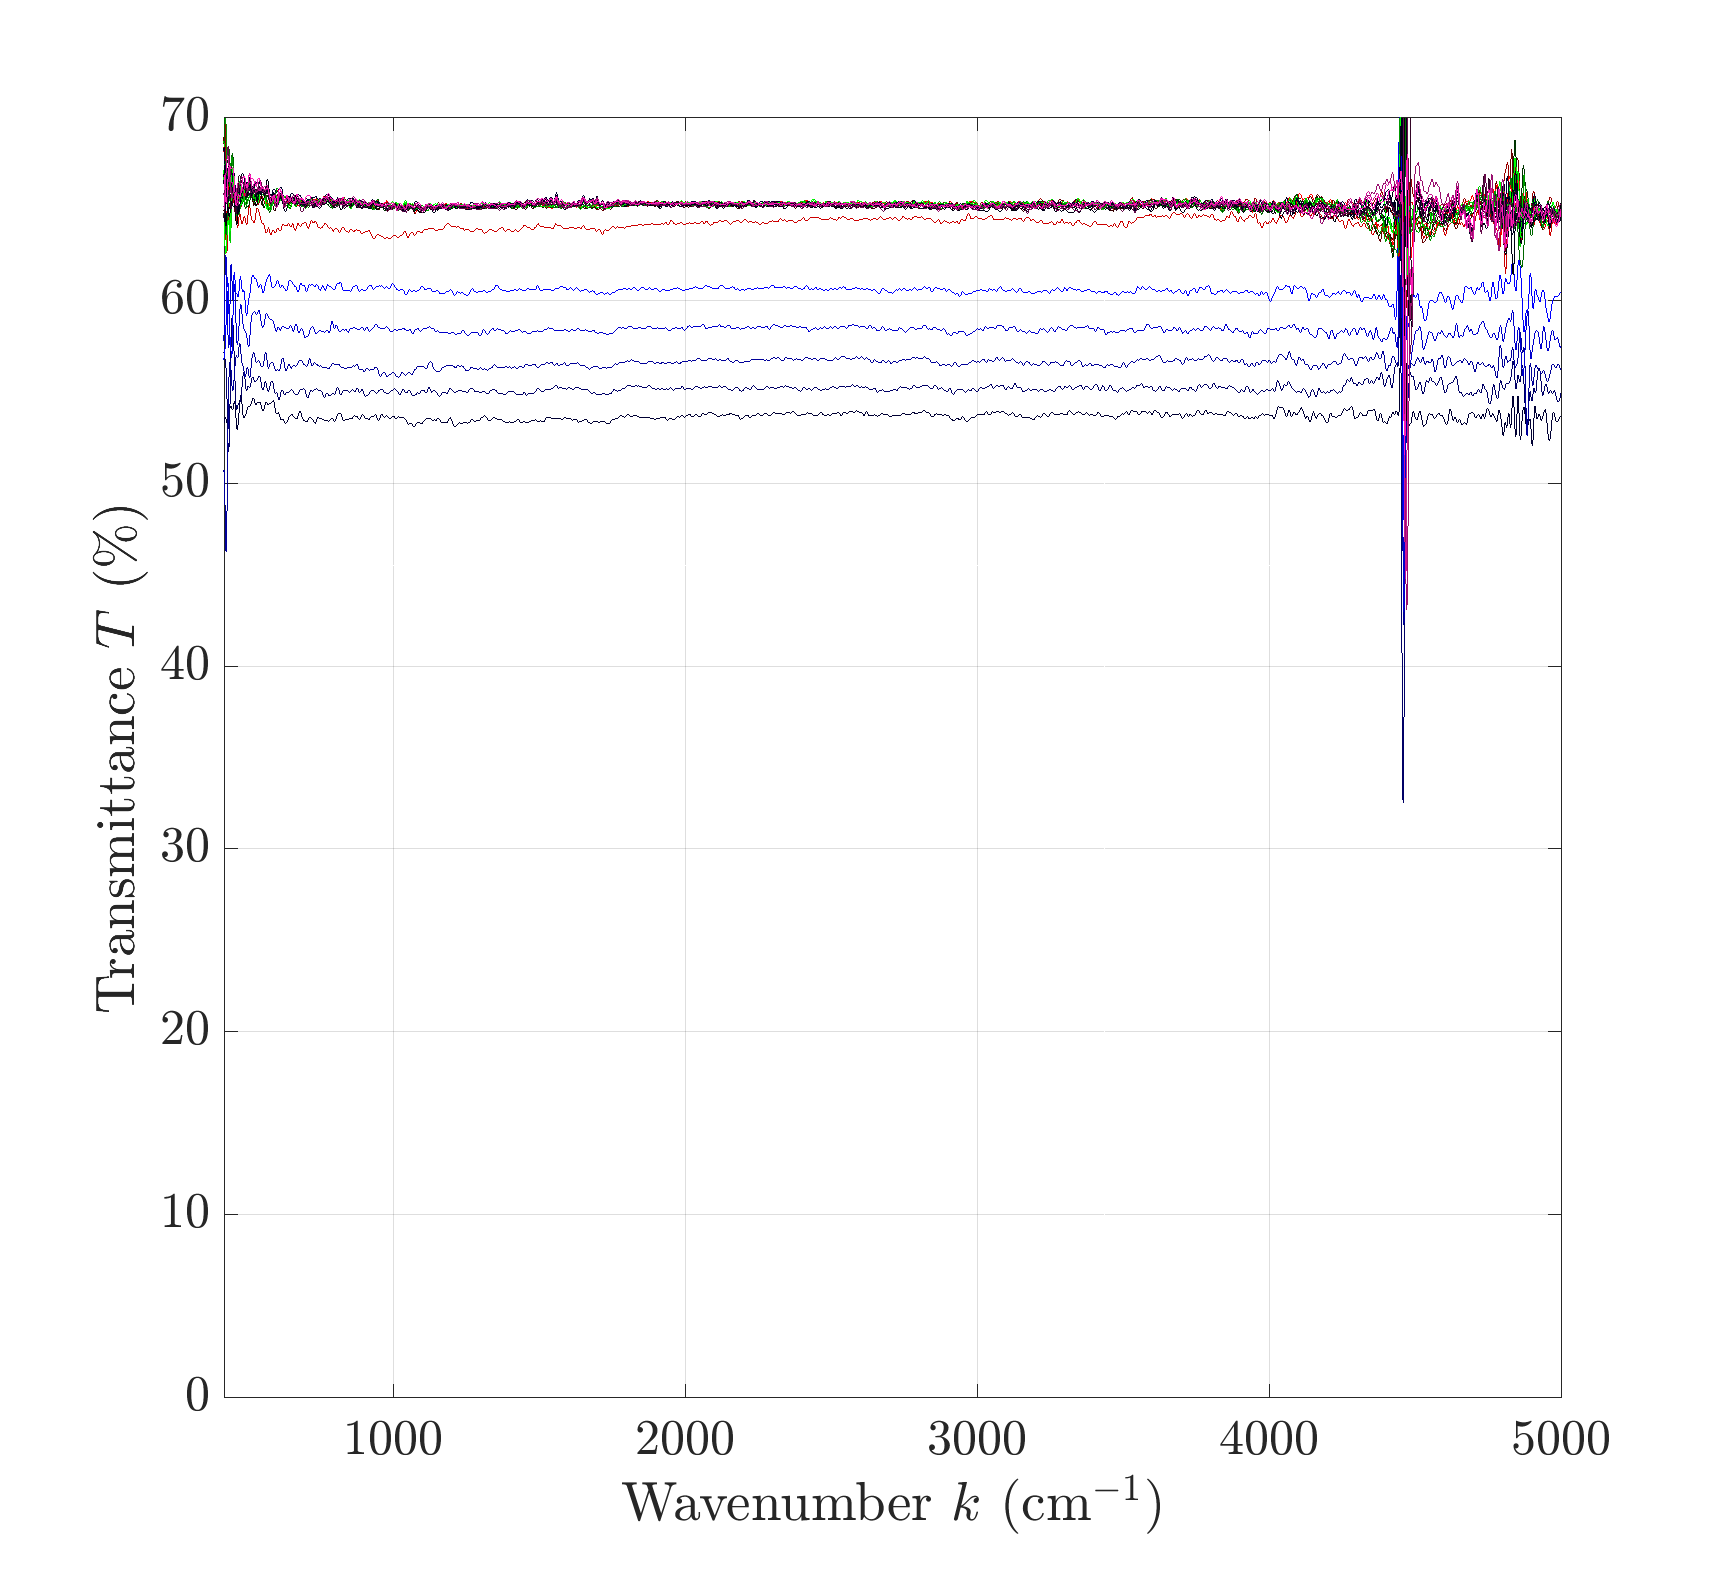
\includegraphics[width=\linewidth]{subCa_25_ftir_spectra.png}
        \caption{}\label{fig:subCa_ftir_spectra}
    \end{subfigure}
    \hfill
    \begin{subfigure}[t]{0.37824561403\linewidth}
        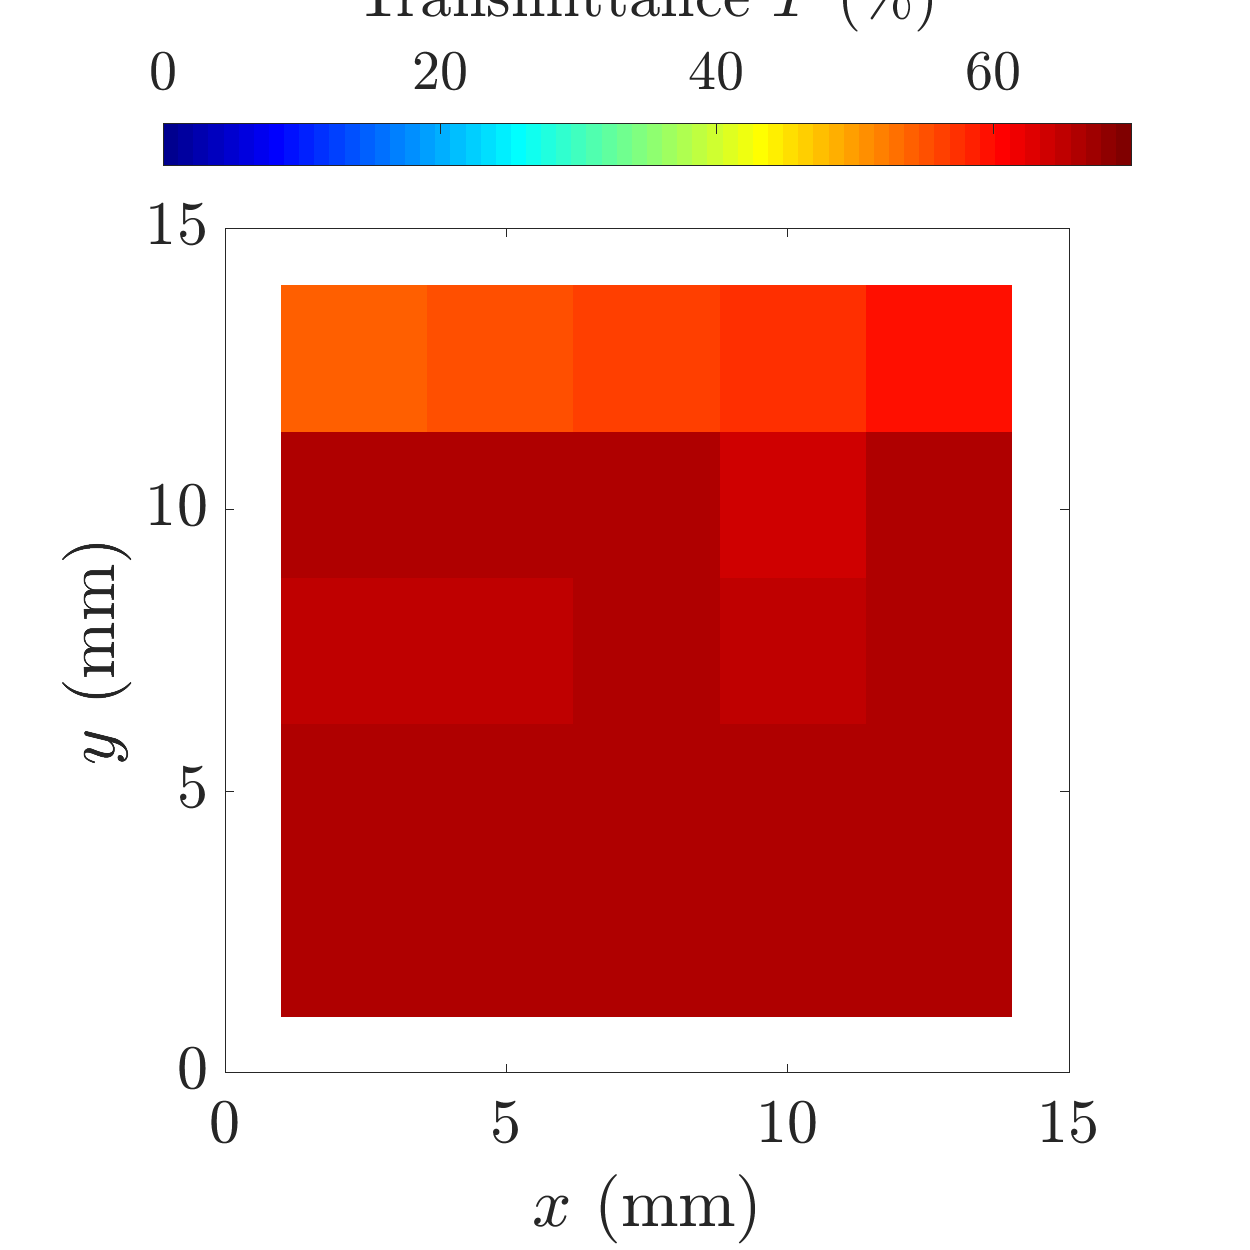
\includegraphics[width=\linewidth]{subCa_25_ftir_transmission_at_k500cm-1.png}
        \caption{}\label{fig:subCa_ftir_map_500cm-1}
    \end{subfigure}
    \caption[\Ac{ftir} measurements of the as-received substrate C.]{\Acf{ftir} measurements recorded from a $5\times5$ grid on the as-received (211)B-oriented substrate C: \subref{fig:subCa_ftir_spectra} Transmission spectra; and \subref{fig:subCa_ftir_map_500cm-1} transmission map at wavenumber $k=\SI{500}{\centi\metre^{-1}}$ showing the transmittance $T$ in percentage of incoming light that is transmitted through at each grid point.}
\end{figure}

The five measurements obtained from the upper edge of substrate C had transmittance between \SI{55}{\percent} and \SI{61}{\percent} in the wavenumber region of interest, which are lower than for the rest of the substrate. Apart from having lower transmission they have the same shape and similar $T_{1000}/T_{5000}$ indicator as the other spectra. For this reason, and the fact that the lower transmission occur in the upper edge, it is believed that the frame that holds the substrate obscure the light at the upper edge, and results in an overall lower transmission (E. Selvig, personal communication, May 24, 2017). Taking this into account, the spectra from the upper edge have the same characteristics as the rest.
%and the indicator $T_{1000}/T_{5000}$ tends to be a little bit larger than one for these points. According to \citet{yujie2004infrared}, the \ac{czt} substrates with these characteristics have a high density of tiny and dense \ce{Te} precipitates, high free carrier concentrations, and a resistivity less than \SI{500}{\ohm\centi\metre}.



%%=========================================